\documentclass{article}
\usepackage[oldvoltagedirection]{circuitikz}
\usepackage[margin=1in, headheight=14pt]{geometry}
\usepackage{amsmath}
\usepackage{mathtools}
\usepackage{graphicx}
\usepackage{karnaugh-map}
\usepackage{fancyhdr}
\setlength\parindent{0pt}

\title{Reti Logiche}
\author{}
\graphicspath{{img/}}

\pagestyle{fancy}

\begin{document}

\maketitle{}

23 Sep 2019, 16:14
\section{Propiet\'a delle reti loiche}


\begin{itemize}
    \item{Intrconnessione}
    \item{Scomposizione}
        Uno schema logico pu\'o essere rappresentato come composizione di reti pi\'u semplici, (si arresta quando si arriva a \textit{reti logiche elemnetari})
    \item{Elementari}
        Descrivono causa effetto
\end{itemize}

Nei sistemi pratici la storia passata del sistema deve essere rappresentata attraverso un insieme finito di segnali. (i.e. il numero passato di stati della rete deve essere finito) (slide 36. 01\_Modelli)

La funzione di uscita della rete dipende da ingresso corrente e stato interno della rete.

\begin{itemize}
    \item{Funzione di uscita o funzione macchina: $z(t) = f(x(t), y(t))$ (tabella, lookup-table)}
    \item{Next step function: $Y(t) = g(x(t), y(t))$, $g(x, y)$ chiamata \textbf{Funzione di stato}}
    \item{Funzione di marcatura dello stato: $y(t + \Delta t) = Y(t)$ o $y(t) = Y(t - \Delta t)$}
\end{itemize}

% Figura slide 40: Modello di mealy, funzioni caratteristiche, (quelle sopra)
\begin{circuitikz}
    \draw (0, 0) node[anchor=east]{x} -- (1, 0) to[twoport, t=$f$, >, number inputs=2] (2, 0) -- (3, 0) node[anchor=west]{z};
\end{circuitikz}

Nelle reti logiche combinatorie manca la dipendena dal tempo (slide 41)

Reti sequenziali corrispondono al modello generale, contengono retroazione e ritardi

% Figura slide 43: Blocco f corisponde ad una rete combinatoria
% Ingresso non cambia facendo cambiare l'uscita, cambia facendo variare le variabili di stato. Una rete di questo modo viene chiamata "Modello di Moore"
% Una rete di questo tipo e' ancora una rete sequenziale

%es:
Rete senza ingressi provenienti dall'eseterno viene chiamata: rete autonoma.  ($y(t) = y(t+1)$: la rete \'e costante).
Altra alternativa \'e un comportamento ciclico.

%%% Guarda se togliere
Se:
$z = f(x)$ e $Y= g(x, y)$: rete combinatoria, dipende solo da $z$


Rete sequenziale con ingresso non attaccato a $g$ \'e rete combinatoria (sostituire con figura)

Rete sequenziale con uscita non attaccata a $g$ \'e rete combinatoria (sostituire con figura)

Sintesi multiuscita pg. 29 slide \_2\_RetiCombinatorie\_I\_parte

Numero funzioni di $n$ variabili $F(n) = 2^{2^n}$, slide 30

\begin{center}
    \begin{tabular}{c c c|c}
        $x_1$ & $x_2$ & $x_3$ & $f$\\
        \hline{}
        0 & 0 & 0 & 0\\
        0 & 0 & 1 & 0\\
        0 & 1 & 0 & 0\\
        0 & 1 & 1 & 1\\
        \hline{}
        1 & 0 & 0 & 0\\
        1 & 0 & 1 & 1\\
        1 & 1 & 0 & 1\\
        1 & 1 & 1 & 1\\
    \end{tabular}
\end{center}

Metodo somma di prodotti: prendo solo righe con 1, le scrivo come prodotti e le sommo

\[
    \begin{rcases}
        f_3 = \overline{x_1} x_2 x_3\\
        f_5 = x_1 \overline{x_2} x_3\\
        f_6 = x_1 x_2 \overline{x_3}\\
        f_7 = x_1 x_2 x_3
    \end{rcases}
    f =  \overline{x_1} x_2 x_3 + x_1 \overline{x_2} x_3 +  x_1 x_2 \overline{x_3} + x_1 x_2 x_3
\]

Applicbile a qualsiasi tabella combinatoria ( Espressione canonica \textit{sum of products} SP)


\subsection{Espressione canonica Prodotto di Somme: PS}

Data una tabella della verit\'a, consideriamo gli zeri della funzione (OFF-set). Per ogni zero possiamo costruire un termine somma in cui compaiono come variabili dipendenti tutte le variabili della funzione di partenza.
Le variabili compaiono in forma vera se compaiono come zeri, vengono prese in forma complementata se compaiono come 1 nella riga della tabella.

\[
    \begin{rcases}
        s_0 = x_1 x_2 x_3\\
        s_1 = x_1 x_2 \overline{x_3}\\
        s_2 = x_1 \overline{x_2} x_3\\
        s_4 = \overline{x_1} x_2 x_3
    \end{rcases}
    S =  (x_1 x_2 x_3)(x_1 x_2 \overline{x_3})(x_1 \overline{x_2} x_3)(\overline{x_1} x_2 x_3)
\]

% Equivalenza espressioni booleane - Reti Combinatorie (Slide 50)
% Manca Conta porte logiche N_op = 5 e N_M = 16
Si riescono a sintetizzare reti pi\'u ottimizzate attraverso le mappe di Karnugh o alg. Quiaf-McCluskeyt

N letterari: si applica su soltanto al max 2 livelli. Conta il numero di morsetti del $1^o$ livello (somma: $N_{let}$ = 12, prodotto 12, altro 6)

\newpage
\section{24 Sep 2019,  9:02}
% Definizione min e max termine slide: reti combinatorie parte 2
Prendendo in considerazione l'esempio del Full-Adder (slide 4)
\subsection{Espressione canonica \textit{SoP} delle funzioni $S_0$ e $C_1$}
$S_0 = \overline{x_0} \overline{y_0} c_1 + \overline{x_0} y_0 \overline{c_0} + x_0 \overline{y_0} \overline{c_0} + x_0 y_0 c_0 = m_1 + m_2 + m_4 + m_7 = \sum m_3(1, 2, 4, 7)$\\
$C_1 = \overline{x_0} y_0 c_0 + x_0 \overline{y_0} c_0 + x_0 y_0 \overline{c_0} + x_0 y_0 c_0 = m_3 + m_5 + m_6 + m_7 = \sum m_3(3, 5, 6, 7)$

Un modo pi\'u preciso sarebbe: $S(x_0, y_0, c_0) $, esplicitando l'ordine in cui vengono prese le variabili

$\sum m_3$ indica la sommatoria dei mintermini di 3 variabili


\subsection{Espressione canonica \textit{PoS}}

$S_0 (x_0, y_0, c_0) = (x_0 + y_0 + c_0) (x_0 + \overline{y_0} + \overline{c_0}) (\overline{x_0} + y_0 + \overline{c_0}) (\overline{x_0} + \overline{y_0} + c_0) = M_0 M_3 M_5 M_6 = \prod M_3(0, 3, 5, 6)$


\subsection{Teorema di Shannon}
Ogni espressione logica di $n$ variabili pu\'o essere espressa come:

\[f(x_1, x_2, \ldots, x_n) = x_1 \cdot f(0, x_2, \ldots, x_n) + x_1 \cdot f(1, x_2, \ldots, x_n)\]

Dall'espressione di una funzione riusciamo a riottenere la somma dei mintermini, utilizzando il th.\ di Shannon:

\[
    \begin{split}
        z &= x_1 x_2 + x_1 x_3 + x_2 x_3 = \\
         &= \overline{x_1} ( 0 \cdot x_2 + 0 x_3 + x_2 x_3) + x_1 (1 x_2 + 1 x_3 + x_2 x_3) = \\
         &= \overline{x_1} (x_2 x_3) + x_1 (x_2 + x_3 + x_2 x_3) = \\
         &= \overline{x_2} (x_1 (0 x_3) + x_1 (0 + x_3 + 0 x_3)) + x_2 (\overline{x_1} (1 x_3) + x_1 (1 + x_2 + 1 x_3)) =\\
         &= \overline{x_2} (x_1 x_3) + x_2 (\overline{x_1} x_3 + x_1) =\\
         &= \overline{x_3} (\overline{x_2} x_1 0 + x_2 \overline{x_1} 0 + x_2 x_1) + x_3 (\overline{x_2} x_1 1 + x_2 \overline{x_1} 1 + x_2 x_1) =\\
         &= \overline{x_2} x_2 x_1 + x_3 \overline{x_2} x_1 + x_3 x_2 \overline{x_1} + x_3 x_2 x_1 =\\
         &= m_3 + m_5 + m_6 + m_7
  \end{split}
  \]


Le leggi di de morgan dimostrano che le famiglie (And-Not) e (Or-Not) sono funzionalmente complete.

% TODO: Immagine circuito
% TODO: Immagine decoder con mintermini
\begin{figure}[ht]
    \begin{circuitikz}[scale=0.7]
    \node at (0, 0) [ocirc](x1){}  (0, 0) node[above]{$X_1$};
    \node at (0.5, 0) [ocirc](x2){}  (0.5, 0) node[above]{$X_2$};
    \node at (1, 0) [ocirc](x3){} (1, 0) node[above]{$X_3$};

    \draw (2, -0.5) node[american and port, anchor=in 1, number inputs=3](N1){};
    \draw (2, -2.5) node[american and port, anchor=in 1, number inputs=3](N2){};
    \draw (2, -4.5) node[american and port, anchor=in 1, number inputs=3](N3){};
    \draw (2, -6.5) node[american and port, anchor=in 1, number inputs=3](N4){};
    \draw (2, -8.5) node[american and port, anchor=in 1, number inputs=3](N5){};
    \draw (2, -10.5) node[american and port, anchor=in 1, number inputs=3](N6){};
    \draw (2, -12.5) node[american and port, anchor=in 1, number inputs=3](N7){};
    \draw (2, -14.5) node[american and port, anchor=in 1, number inputs=3](N8){};

    %\draw (0.5, 0) node[anchor=south]{$x_2$} --(0 |- N8.in 2);
    %\draw (1, 0) node[anchor=south](x3){$x_3$} --(1, -14.5);
    \draw (x1) --(x1 |- N8.in 1);
    \draw (x2) --(x2 |- N8.in 2);
    \draw (x3) --(x3 |- N8.in 3);

    \draw (x1 |- N1.in 1) to[short, *-] (N1.in 1);
    \draw (x2 |- N1.in 2) to[short, *-] (N1.in 2);
    \draw (x3 |- N1.in 3) to[short, *-] (N1.in 3);

    \draw (x1 |- N2.in 1) to[short, *-] (N2.in 1);
    \draw (x2 |- N2.in 2) to[short, *-] (N2.in 2);
    \draw (x3 |- N2.in 3) to[short, *-] (N2.in 3);

    \draw (x1 |- N3.in 1) to[short, *-] (N3.in 1);
    \draw (x2 |- N3.in 2) to[short, *-] (N3.in 2);
    \draw (x3 |- N3.in 3) to[short, *-] (N3.in 3);

    \draw (x1 |- N4.in 1) to[short, *-] (N4.in 1);
    \draw (x2 |- N4.in 2) to[short, *-] (N4.in 2);
    \draw (x3 |- N4.in 3) to[short, *-] (N4.in 3);

    \draw (x1 |- N5.in 1) to[short, *-] (N5.in 1);
    \draw (x2 |- N5.in 2) to[short, *-] (N5.in 2);
    \draw (x3 |- N5.in 3) to[short, *-] (N5.in 3);

    \draw (x1 |- N6.in 1) to[short, *-] (N6.in 1);
    \draw (x2 |- N6.in 2) to[short, *-] (N6.in 2);
    \draw (x3 |- N6.in 3) to[short, *-] (N6.in 3);

    \draw (x1 |- N7.in 1) to[short, *-] (N7.in 1);
    \draw (x2 |- N7.in 2) to[short, *-] (N7.in 2);
    \draw (x3 |- N7.in 3) to[short, *-] (N7.in 3);

    \draw (x1 |- N8.in 1) to[short, *-] (N8.in 1);
    \draw (x2 |- N8.in 2) to[short, *-] (N8.in 2);
    \draw (x3 |- N8.in 3) to[short, *-] (N8.in 3);

    \node at (N1.bin 1) [ocirc, left]{};
    \node at (N1.bin 2) [ocirc, left]{};
    \node at (N1.bin 3) [ocirc, left]{};

    \node at (N2.bin 1) [ocirc, left]{};
    \node at (N2.bin 2) [ocirc, left]{};

    \node at (N3.bin 1) [ocirc, left]{};
    \node at (N3.bin 3) [ocirc, left]{};

    \node at (N4.bin 1) [ocirc, left]{};

    \node at (N5.bin 2) [ocirc, left]{};
    \node at (N5.bin 3) [ocirc, left]{};

    \node at (N6.bin 1) [ocirc, left]{};
    \node at (N6.bin 3) [ocirc, left]{};

    \node at (N7.bin 3) [ocirc, left]{};
\end{circuitikz}

    \centering
    \caption{Decoder 3:8 ad AND}
\end{figure}

DECODER: ad $n$ ingresi corrispondono $2^n$ uscite

% TODO: Immagine decoder con MAXTERMINI (Decoder 3:8 a OR)
% TODO: De morgan con OR (ingresso al centro negato) -> AND negati invertiti
% Simbolo nand si puo fare con frecce
% TODO: Decoder a nand (produce MAXTERMINI)

\textbf{Espressione generale SP}: $f(x_{n-1}, \ldots, x_1, x_0) = \sum_{i=0, 2^n -1} m(i) f(i)$

\textbf{Espressione generale PS}: $f(x_{n-1}, \ldots, x_1, x_0) = \prod_{i=0, 2^n -1} (M(i) +f(i))$

%TODO: foto multiplexer a 8 canali con 3 var di selezione del canale Aggiungendo valori della funzione con carry out guarda foto
Il decoder sta in corrispondenza con le espressioni canoniche, il multiplexer sta un corrispondenza con le espressioni generali.


\newpage
\section{25 Sep 2019, 14:46}
%TODO: Immagine 1

\begin{itemize}
    \item{Il segnale RC ($RC_0$ e $RC_1$) dipendono da $n-1$ variabili. e non da $n$ variabili.}
    \item{$RC_0$ e $RC_1$ potrebbero essere semplificabili}
\end{itemize}

Una funzione di n variabili pu\'o essere espressa come una combinazione di due funzioni di n-1 variabili attraverso un Multiplexer.
\[f(x_1, x_2, \ldots, x_n) = \overline{x_1}\overline{x_2} f(0, 0, \ldots, x_n) + \overline{x_1} x_2 f(0, 1, \ldots, x_n) + x_1 \overline{x_2} f(1, 0, \ldots, x_n) + x_1 x_2 f(1, 1, \ldots, x_n)\]

Funzione semplificata di due variabili con Th.\ di Shannon.
%TODO: Immagine 2


\begin{minipage}{0.4\textwidth}
\begin{center}
    \begin{karnaugh-map}[4][4][1][$C D$][$A B$]
        \minterms{1,4,5,6,7,12,15,14,9}
        \autoterms[0]

        \implicant{0}{2}
        \implicant{4}{6}
        \implicant{12}{14}
        \implicant{8}{10}
    \end{karnaugh-map}
\end{center}
\end{minipage}
\begin{minipage}{0.4\textwidth}
\[
    \begin{split}
        f_0 &= \overline{C} D\\
        f_1 &= 1\\
        f_3 &= C + \overline{D}\\
        f_2 &= \overline{C} D
    \end{split}
\]
\end{minipage}

\begin{minipage}{0.4\textwidth}
\begin{center}
    \begin{karnaugh-map}[4][4][1][$C D$][$A B$]
        \minterms{1,4,5,6,7,12,15,14,9}
        \autoterms[0]

        \implicant{0}{6}
        \implicant{12}{10}
    \end{karnaugh-map}
\end{center}
\end{minipage}
\begin{minipage}{0.4\textwidth}
\[
    \begin{split}
        f_0 &= B + \overline{C} D\\
        f_1 &= B \overline{D} + BC + \overline{B}\overline{C}D
    \end{split}
\]
\end{minipage}

Supponendo di dover realizzare la funzione con un multiplexer a 4 vie, utilizzando esclusivamente un mux e non altri componenti:

%TODO: Immagine  (3 mux a 4 vie)

Nel caso in cui fossimo partiti dalle variabili $CD$:

%TODO: Stessa mappa k con raccoglimenti verticali
\[
    \begin{split}
        f_0 &= B\\
        f_1 &= \overline{A} + \overline{B} = \overline{A\cdot B}\\
        f_2 &= B\\
        f_3 &= B
    \end{split}
\]

\begin{itemize}
    \item Espressione canonica SP
        \begin{itemize}
            \item AND per mintermini + OR
            \item Decoder + or
        \end{itemize}
    \item Espressione canonica PS
        \begin{itemize}
            \item OR per Maxtermini + AND
            \item Decoder a NAND + AND
        \end{itemize}
    \item Espressione generale SP e PS: MuX
    \item Espressione parziali: (1 MUx + altro)
\end{itemize}

\begin{tabular}{c c c| c c}
    a & b & c & Sum & Count\\
    \hline
    0 & 0 & 0 & 0 & 0\\
    0 & 0 & 1 & 1 & 0\\
    0 & 1 & 0 & 1 & 0\\
    0 & 1 & 1 & 0 & 1\\
    1 & 0 & 0 & 1 & 0\\
    1 & 0 & 1 & 0 & 1\\
    1 & 1 & 0 & 0 & 1\\
    1 & 1 & 1 & 1 & 1\\
\end{tabular}


$\text{Count} = \overline{a}b c + a\overline{b} c + a b \overline{c} + a b c = \overline{a} b c + a \overline{b} c + ab$

\[
    \begin{cases}
        N_{op} = 5\\
        N_m = 3 \cdot 4 + 4 = 16
    \end{cases} \to
    \begin{cases}
        N_{op} = 4\\
        N_m = 11
    \end{cases}
\]

Definiamo come \textbf{distanza di Hamming} ($\mathcal{D}_H$) il numero di bit che differiscono in 2 configurazioni binarie

Es: $\mathcal{D}_H ( 1 1 0, 1 1 1) = 1$

Se $\mathcal{D}_H (C_i, C_j) = 1 \Rightarrow C_i\, \text{e}\, C_j$ sono \textbf{adiacenti}.

% Slide 20

\begin{center}
\begin{karnaugh-map}[4][2][1][$bc$][$a$]
    \minterms{3,5,6,7}
    \autoterms[0]
    \implicant{5}{7}
    \implicant{7}{6}
    \implicant{3}{7}
\end{karnaugh-map}
\end{center}

Raggruppamento rettangolare di 2 caselle $2^1$ caselle ($2^k = 2^1$) (Raggruppamento di ordine 1)

% Slide 23
$C_{out} = I_1 + I_2 + I_3 = ac + ab + bc$ \qquad($N_{op} = 4 , N_m = 9$)


\begin{center}
    \begin{karnaugh-map}[4][4][2][$cd$][$ab$][$E$]
        \minterms{1,4,5,6,7,12,14,15,9}
        \indeterminants{13}

        %E = 1
        \minterms{20,28,25,31}
        \indeterminants{16,18,30,26,29,23}
        \autoterms[0]

        \implicant{1}{9}
        \implicant{4}{14}
        \implicant{12}{14}[0,1]
        \implicant{13}{9}[0,1]
        \implicant{4}{12}[0,1]
    \end{karnaugh-map}
\end{center}
$Z(a, b, c, d ,e)$

'-' rappresenta una condizione di indifferenza.

Nei raggruppamenti prendo in considerazione le variabili che rimangono costanti

\[
    Z(a, b, c, d ,e) = b\overline{e} + \overline{c}d\overline{e} + b \overline{c}\overline{d} + a \overline{c}d + ab
\]


$N_{lett} = 13$, ingressi del primo livello

$N_{op} = 6$, numero mintermini + 1

$N_m = 18$, tutte le lettere che compaiono + mintermini

% TODO: Raggruppa come in figura 6
\subsection{Sintesi prendendo in considerazione gli zeri}
Uno 0 di una funzione \'e un maxtermine, ed esprime un solo 0. L'obbiettivo \'e costruire termini somma (Implicati)

\begin{center}
    \begin{karnaugh-map}[4][4][2][$cd$][$ab$][$E$]
        \minterms{1,4,5,6,7,12,14,15,9}
        \indeterminants{13}

        %E = 1
        \minterms{20,28,25,31}
        \indeterminants{16,18,30,26,29,23}
        \autoterms[0]

        \implicantcorner[0,1]
        \implicantedge{3}{2}{11}{10}[0,1]
        \implicant{17}{23}
        \implicant{19}{22}
    \end{karnaugh-map}
\end{center}

\[ Z = (B + \overline{C})(A + \overline{D} + \overline{E})(\overline{C} + D + \overline{E})(B + D) = (B \downarrow \overline{C}) \downarrow (A\downarrow \overline{D}\downarrow\overline{E})\downarrow(\overline{C}\downarrow D\downarrow \overline{E})\downarrow (B\downarrow D)\]

$N_{op} = 5$

$N_{m} = 14$

Sintesi di $Z(A, B, C, D, E) $

\begin{itemize}
    \item mediante soli MUX a 4 vie
    \item 1 porta logica + MUX a 4 vie
\end{itemize}

%TODO: figura 6
\section{lezione 30 Sep 2019, 14:38}
Es:

\begin{center}
    \begin{karnaugh-map}[4][4][2][$X_0 X_1$][$X_3 X_2$][$X_4$]
        \minterms{1,2,3,5,7,11,13,17,19,23,29,31}
        \autoterms[0]
        \implicant{3}{2}
        \implicant{1}{3}[0,1]
        \implicant{29}{31}
        \implicant{5}{13}
        \implicant{5}{7}
        \implicant{23}{23}
        \implicantedge{3}{3}{11}{11}
    \end{karnaugh-map}
\end{center}

\[
    Z =
    \overline{x_4}\overline{x_3}\overline{x_2} \overline{x_3}\overline{x_2}x_0
    +\overline{x_3}\overline{x_2}x_0
    + \overline{x_4}\overline{x_2}x_1 x_0 +
    + x_4 x_3 x_2 x_0 + \overline{x_3} x_2 x_1 x_0 + \overline{x_4} x_2 \overline{x_1} x_0
\]

\[N_b = 7 \qquad N_m = 29\]


Operatore NAND: $x_1 \uparrow x_2 \uparrow \ldots \uparrow x_n = \overline{x_1 \cdot x_2 \cdot \ldots \cdot x_n}$

Operatore NOR: $x_1 \downarrow x_2 \downarrow \ldots \downarrow x_n = \overline{x_1 + x_2 + \ldots + x_n}$

(Non vale la proprietà associativa)

(Completezza funzionale NAND lezione 5 slide 6)

(Completezza funzionale NAND lezione 5 slide 7)

\begin{center}
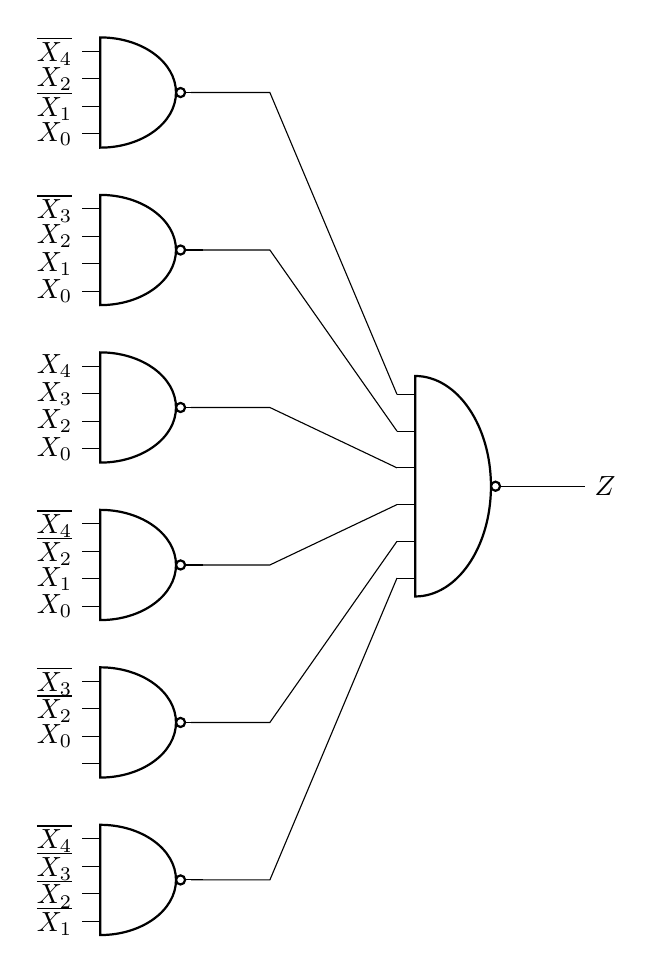
\begin{tikzpicture}
    \begin{scope}
        \ctikzset{tripoles/american nand port/height=2}
        \draw(4, 5) node[american nand port, number inputs=6](coll){} -- ++(1, 0) node[right]{$Z$};
    \end{scope}
    \begin{scope}
        \ctikzset{tripoles/american nand port/height=1}
        \draw (0, 0) node[american nand port, number inputs=4](p1){} -- ++(1, 0) -- (coll.in 6);
        \draw (0, 2) node[american nand port, number inputs=4](p2){} -- ++(1, 0) -- (coll.in 5);
        \draw (0, 4) node[american nand port, number inputs=4](p3){} -- ++(1, 0) -- (coll.in 4);
        \draw (0, 6) node[american nand port, number inputs=4](p4){} -- ++(1, 0) -- (coll.in 3);
        \draw (0, 8) node[american nand port, number inputs=4](p5){} -- ++(1, 0) -- (coll.in 2);
        \draw (0, 10) node[american nand port, number inputs=4](p6){} -- ++(1, 0) -- (coll.in 1);
    \end{scope}

    \draw (p1.in 1) node[left]{$\overline{X_4}$};
    \draw (p1.in 2) node[left]{$\overline{X_3}$};
    \draw (p1.in 3) node[left]{$\overline{X_2}$};
    \draw (p1.in 4) node[left]{$\overline{X_1}$};

    \draw (p2.in 1) node[left]{$\overline{X_3}$};
    \draw (p2.in 2) node[left]{$\overline{X_2}$};
    \draw (p2.in 3) node[left]{$X_0$};

    \draw (p3.in 1) node[left]{$\overline{X_4}$};
    \draw (p3.in 2) node[left]{$\overline{X_2}$};
    \draw (p3.in 3) node[left]{$X_1$};
    \draw (p3.in 4) node[left]{$X_0$};

    \draw (p4.in 1) node[left]{$X_4$};
    \draw (p4.in 2) node[left]{$X_3$};
    \draw (p4.in 3) node[left]{$X_2$};
    \draw (p4.in 4) node[left]{$X_0$};

    \draw (p5.in 1) node[left]{$\overline{X_3}$};
    \draw (p5.in 2) node[left]{$X_2$};
    \draw (p5.in 3) node[left]{$X_1$};
    \draw (p5.in 4) node[left]{$X_0$};

    \draw (p6.in 1) node[left]{$\overline{X_4}$};
    \draw (p6.in 2) node[left]{$X_2$};
    \draw (p6.in 3) node[left]{$\overline{X_1}$};
    \draw (p6.in 4) node[left]{$X_0$};
\end{tikzpicture}
\end{center}
È possibile convertire un qualsiasi circuito logico utilizzando soli NAND.

Costo del circuito semplificato: $N_m = 29$, esattamente uguale a quello con operatori booleni, il costo $N_m$ e $N_b \coloneqq N_{op}$ è esattamente lo stesso

\subsection{Come passare da SP a NAND}
Lezione 5 slide 8

\begin{enumerate}
    \item Involuzione: doppia negazione
    \item Trasformo dell'involuzione con De Morgan
\end{enumerate}

Es.
\[
    \begin{split}
        Z &= \bar{a} + a \bar{b} + a\bar{b}\bar{c} + ab\bar{c} \\
        &= \overline{\overline{( \bar{a} + a \bar{b} + a\bar{b}\bar{c} + ab\bar{c} )}}\\
        &= \overline{a \cdot (a \uparrow \bar{b}) \cdot(a \uparrow \bar{b} \uparrow \bar{c}) \cdot (a \uparrow b \uparrow \bar{c})} \\
        &= a \uparrow (a \uparrow \bar{b}) \uparrow(a \uparrow \bar{b} \uparrow \bar{c}) \uparrow (a \uparrow b \uparrow \bar{c})
    \end{split}
\]

(Slide 10 punto 4 ultimo b è negato)

NOTA: MAI sintetizzare una rete NOR partendo da SP
\subsection{Trasformazione a NAND in rete a più livelli}
\begin{enumerate}
    \item Inserire le parentesi sottintese
    \item Numerare i livelli
    \item Trasformare gli operatori AND e OR in NAND
    \item Complementare eventuali letterari isolati che costituiscono variabili di funzioni OR (tutte a livello pari)
\end{enumerate}

\subsection{Trasformazione a NOR in rete a più livelli}
\begin{enumerate}
    \item Inserire le parentesi sottintese
    \item Numerare i livelli
    \item Trasformare gli operatori AND e OR in NOR
    \item Complementare eventuali letterari isolati che costituiscono variabili di funzioni AND (tutte a livello dispari)
\end{enumerate}

\[ Z  = (b \uparrow ( \overline{d} \uparrow  e)) \uparrow (\overline{c} \uparrow (1 \uparrow (\overline{d} \uparrow c))) \uparrow a \]

Operatori a livello dispari: Somme, pari: prodotti

\[ = ( b \cdot (d + \overline{e}))  + (\overline{c} \cdot ( 0 + (\overline{d} \cdot e))) + \overline{a} = \]
\[ = bd + b \overline{e} + \overline{c}\overline{d}e + \overline{a} \]

\begin{center}
    \begin{karnaugh-map}[4][4][2][$ab$][$cd$][$e$]
        \maxterms{8,9,10,11,25,26,27,30}
        \autoterms[1]
        \implicant{8}{10}
        \implicant{9}{11}[0,1]
        \implicant{30}{26}
    \end{karnaugh-map}
\end{center}
\[
    Z = (e + \overline{a} + b)(\overline{e} + \overline{c} + d + \overline{a}) (\overline{a} + b + \overline{d})
    = (e \downarrow \overline{a} \downarrow b) \downarrow (\overline{e} \downarrow \overline{c} \downarrow d \downarrow \overline{a}) \downarrow
    (\overline{a} \downarrow b \downarrow \overline{d})
\]


\subsection{Esercizio prova passata d'esame}
Realizzare la funzione sotto riportata. Utilizzando solamente i componenti a disposizione (4 nand + variabili in forma negata)

\[ F = x y \overline{z} + \overline{x} y \overline{x} \overline{w} + x y z \overline{w} + \overline{x} y z \]
\begin{center}
    \begin{karnaugh-map}[4][4][1][{$xy$}][{$zw$}]
        \minterms{12,4,7,6,14,13}
        \autoterms[0]
        \implicantedge{4}{12}{6}{14}
        \implicant{12}{13}
        \implicant{7}{6}
    \end{karnaugh-map}
\end{center}
\[
    F = y\overline{w} + \overline{x} yz  + x y \overline{z} = (y \uparrow \overline{w}) \uparrow (\overline{x} \uparrow y \uparrow z) \uparrow (x \uparrow y \uparrow \overline{z})
\]


% TODO: figura con righe colorate
\begin{circuitikz}
    \draw (0, 0) node[left]{$x$} --(3, 0) node[](x){};
    \draw (1, 0) -- ++(0, -0.5) -- ++(1, 0) node[american not port, anchor=in, scale=0.6](n1){};
    \draw (n1.out) -- (3, -0.5) node[](nx){};

    \draw (0, -1) node[left]{$y$} --(3, -1) node[](y){};
    \draw (1, -1) -- ++(0, -0.5) -- ++(1, 0) node[american not port, anchor=in, scale=0.6](n2){};
    \draw (n2.out) -- (3, -1.5) node[](ny){};

    \draw (0, -2) node[left]{$z$} --(3, -2) node[](z){};
    \draw (1, -2) -- ++(0, -0.5) -- ++(1, 0) node[american not port, anchor=in, scale=0.6](n3){};
    \draw (n3.out) -- (3, -2.5) node[](nz){};

    \draw (0, -3) node[left]{$y$} --(3, -3) node[](w){};
    \draw (1, -3) -- ++(0, -0.5) -- ++(1, 0) node[american not port, anchor=in, scale=0.6](n4){};
    \draw (n4.out) -- (3, -3.5) node[](nw){};

    \draw (5, -1.75) node[american nand port, number inputs=3](nand1){};
\end{circuitikz}

\subsubsection{Realizzare F con soli MUX a 4 vie ( 2 var di selezione)}

% TODO: Circuito con mux 2:4

\subsubsection{Usando un MUX  a 3 variabili di selezione + altro}
%TODO: circuito con MUX 3:8


\section{Lezione 01 Oct 2019,  9:08}
\subsection{Conversione da realizzazione NAND a NOR e viceversa}
Conversione da SP a NAND-NAND
\[ Z = a \overline{b} \Leftrightarrow Z = (a \overline{b}) + 0 = (a \uparrow \overline{b}) \uparrow 1\]

Conversione PS a NOR-NOR
\[ Z = a \cdot b = \overline{a} \downarrow \overline{b} \]


\[ Z = \overline{a} + b  = a \uparrow \overline{b}\]

\[ Z = (\overline{a} + b)\cdot 1  = (\overline{a} \downarrow b) \downarrow 0 \]

%TODO: Circuito xor a NAND

Metodo \textbf{Standard}:
\begin{enumerate}
    \item Da schama ad espressione NAND
    \item espressione NAND a espressione booleana (SP)
    \item Valutazione tramite mappa K
    \item Resintesi PS
    \item Da PS a NOR (Schema NOR)
\end{enumerate}



\[ Z = ((x\uparrow y) \uparrow x) \uparrow ((x \uparrow y )\uparrow y) \]
\[ Z = ( \overline{x} + \overline{y}) \cdot x + (\overline{x} + \overline{y}) \cdot y = x\overline{y} + \overline{x} y \]

\begin{minipage}{0.5\textwidth}
    \begin{center}
        \begin{karnaugh-map}[2][2][1][{$Y$}][{$X$}]
            \minterms{1,2}
            \autoterms[0]
            \implicant{0}{0}
            \implicant{3}{3}
        \end{karnaugh-map}
    \end{center}
\end{minipage}
\begin{minipage}{0.4\textwidth}
    \[ Z = (x + y) (\overline{x} + \overline{y}) = (x \downarrow y) \downarrow (\overline{x} \downarrow \overline{y})\]
\end{minipage}

\subsection{Proprietà di Dualità}
Da ogni realizzazione booleana se ne ricava un'altra, \underline{duale}, sostituendo AND $\leftrightarrow$ OR (Espressione duale) (Non si toccano i complementi)

Espressione duale viene indicata con $E^D$

NOTA:
\[ E(x, y, z) \rightarrow E^D (x, y, z) \neq E(x, y, z) \]
\subsection{Teorema di dualità}
Se ho un'espressione $Z = f(x_1, x_2, \ldots, x_n)$, allora $Z^D = \overline{f}(\overline{x_1}, \overline{x_2}, \ldots ,\overline{x_n})$.

Inoltre la proprietà di dualità soddisfa l'involuzione: ${(Z^D)}^D = Z$

\subsection{Conversione NAND $\to$ NOR (o viceversa) mediante dualità}
\begin{itemize}
    \item Ricavo espressione duale
    \item Applico teorema dualità
\end{itemize}

\[Z^D = ((x\downarrow y) \downarrow x) \downarrow (( x\downarrow y) \downarrow y)\]
\[ Z = {(Z^D)}^D = \overline{((\overline{x} \downarrow \overline{y}) \downarrow \overline{x} ) \downarrow (\overline{x} \downarrow \overline{y} ) \downarrow \overline{y})} \]

% TODO: disegno XOR con ingresso 0 (out Z^d)

\subsection{Esercizio esame}
Data la funzione delle seguente variabili $Z(x_4, x_3, x_2, x_1, x_0) = \sum m_5(1, 2, 3, 4, 5, 11, 13, 17, 23, 24, 25, 27, 31) + d_5(6, 10, 12, 18, 20, 21, 22, 30)$
\begin{enumerate}
    \item Trascrivere la funzione sulla mappa K
    \item Ricavare l'espressione NOR ottima priva di Alee e riportare il costo in $N_{lett}$
    \item Usare esclusivaente NOR  a 3 ingressi e NOT (schema logico, costo N letterali)
    \item Ricavare una realizzazione di $Z$ basata su un MUX a 3 var di selezione + altro
\end{enumerate}

\begin{center}
    \begin{karnaugh-map}[4][4][2][$X_0 X_1$][$X_2 X_3$][$X_4$]
        \minterms{1,2,3,4,5,11,13,17,23,24,25,27,31}
        \indeterminants{6,10,12,18,20,21,22,30}
        \autoterms[0]
        \implicant{0}{0}[0,1]
        \implicant{7}{14}
        \implicant{8}{9}
        \implicant{20}{29}
        \implicant{19}{18}
        \implicant{14}{10}[0,1]
    \end{karnaugh-map}
\end{center}

\[
    \begin{split}
        Z &= (x_4 + \overline{X_2} + \overline{X_1})(x_4 + \overline{X_3} + X_2 + X_1)( \overline{X_4} + \overline{X_2} + X_1) (\overline{X_4} + X_3 + x_2 + \overline{X_1})(X_3 + X_2 + X_1 + X_0)(\overline{X_4} + \overline{X_3} + X_0))\\
          &= (x_4 \downarrow \overline{X_2} \downarrow \overline{X_1})\downarrow(x_4 \downarrow \overline{X_3} \downarrow X_2 \downarrow X_1)\downarrow( \overline{X_4} \downarrow \overline{X_2} \downarrow X_1)\downarrow (\overline{X_4} \downarrow X_3 \downarrow x_2 \downarrow \overline{X_1})\downarrow(X_3 \downarrow X_2 \downarrow X_1 \downarrow X_0)\downarrow(\overline{X_4} \downarrow \overline{X_3} \downarrow X_0))
      \end{split}
\]

    Elenco componenti utilizzati:
$N_{lett} = 21$
\begin{itemize}
    \item    3 NOR a 3 ingressi
    \item    3 NOR a 1 ingressi
    \item    1 NOR a 6 ingressi
\end{itemize}

% TODO:
% Punto 3
Elenco componenti punto 3:
\begin{itemize}
    \item    6 NOR a 3 ingrressi
    \item    3 NOR a 2 ingrressi
    \item    2 NOR a 3 ingrressi
    \item    1 NOR a 2 ingrressi
    \item    5 NOT
\end{itemize}

Costo in letterari (NOTA: la rete non è più a 2 livelli, per calcolare il costo lo calcolo 'a pezzi di 2 livelli'):

$N_{lett} = N_{lett_a} + N_{lett_b} + N_{lett_c} = 9 + 12 +4 = 25$

%4
\begin{itemize}
    \item Partire sempre dal MUX che pilota l'uscita
\end{itemize}



\end{document}
